%!TEX root = ../documentation.tex

\chapter{Einsatzbereiche}
\section{Norbert - Wie kommt er in das Leben eines Studierenden?}
Norbert - Your StudyBuddy ist eine Anwendung zum Optimieren des Studienalltags, doch wie werden die Studierenden darauf aufmerksam?
Um Norbert bekannt zu machen und die Vorteile der Software zu verbreiten, existieren verschiedene Marketingstrategien die in den nächsten Unterkapiteln vorgestellt werden. Spätestens ab dem ersten Studientag kann der Studierende über die Kurskennung einem virtuellen Kurs beitreten, sich mit anderen Studierenden vernetzten und aktiv Wissensmanagement und Zeitmanagement betreiben.

\subsection{Das duale Partnerunternehmen}
Die dualen Partnerunternehmen sind meistens die ersten Anlaufstellen der Studierenden. Im Vorpraktikum wird  - soweit möglich - bei den höheren Semestern nachgefragt, auf welche Aspekte man in den ersten Semestern achten muss. Doch meistens gestaltet sich dies nicht immer als einfach, denn der Austausch von Dokumenten oder speziellen ToDo's im neuen Semester, haben sich auch die höheren Semester nicht mehr behalten. An diesen Punkten setzt Norbert ein: Das Partnerunternehmen oder die duale Studienvertretung im Unternehmen macht auf die Anwendung aufmerksam. Und kann darüber zentral alle wichtigen Informationen weitergeben. Zudem könnten die Partnerunternehmen als mögliche Hoster der Anwendung in Frage kommen und würden somit die Verwaltung der Anwendung übernehmen.

\textit{Warum sollte eine Firma die Anwendung auf eigene Kosten hosten?}

Gerade in den ersten Semestern wird das Lernpensum gerne unterschätzt, Aufgaben vergessen, Termine und Fristen nicht eingehalten. Dies führt häufig dazu das bereits nach dem ersten Semester bis zu 50\% der dualen Studierenden ihr Studium abbrechen müssen und das Partnerunternehmen verlassen. Das investierte Geld der Unternehmen und wichtige zukünftige Mitarbeiter sind damit verloren.

\subsection{Die Duale Hochschule \& Studienvertretung}
Die Duale Hochschule könnte wie die Partnerunternehmen als Hoster der Anwendung in Frage kommen. Durch die Vermarktung der Software auf der DHBW-Webseite oder bei Studieninformationstagen kann bereits früh auf die neue Software aufmerksam gemacht werden. Außerdem können über diese Anwendung wichtige DHBW-Pressemitteilungen schnell und kostengünstig verbreitet werden. Nicht zu verachten ist auch, dass die Möglichkeit besteht, dass die Durchfallquoten der DHBW sinken und dadurch mehr Partnerunternehmen, besser Zuschüsse und ein allgemein höheres Ansehen erzeugt werden kann.

Die Studienvertretung kann ähnlich wie die DHBW über die Anwendung über Tagungen, Wahlen, Mitteilungen und Kneipentouren informieren und kommt als potentieller Hoster in Frage.

\section{Norbert - Welchen Vorteil bietet er?}
Norbert hilft den Studierenden den Studienalltag besser zu organisieren. Insbesondere hilft Nobert - Your StudyBuddy in folgenden Aspekten:
\begin{enumerate}
	\item Wissensmanagement: Er erinnert die Studierenden an wichtige Termine und lässt sie keine Information mehr vergessen
	\item Wissensweitergabe: Durch die Möglichkeit Aufgaben, Dokumente und Informationen automatisch an Studienkollegen weiterzugeben, kann jeder Studierende selbst aktiv dafür sorgen, dass jeder immer und überall top informiert ist.
	\item Zeitmanagement: Durch die bessere und einfachere Planung des Alltags hat der Student mehr Zeit für Kneipentouren und Partys.	
\end{enumerate}

Die folgende Abbildung verdeutlicht welche Informationen, Termine und Aufgaben der Studierende verpasst haben könnte. Mit Norbert - Your StudyBuddy wäre dies nicht passiert.

\newpage
\begin{landscape}
\vspace*{35mm}
	\begin{figure}[H]
	\centering
	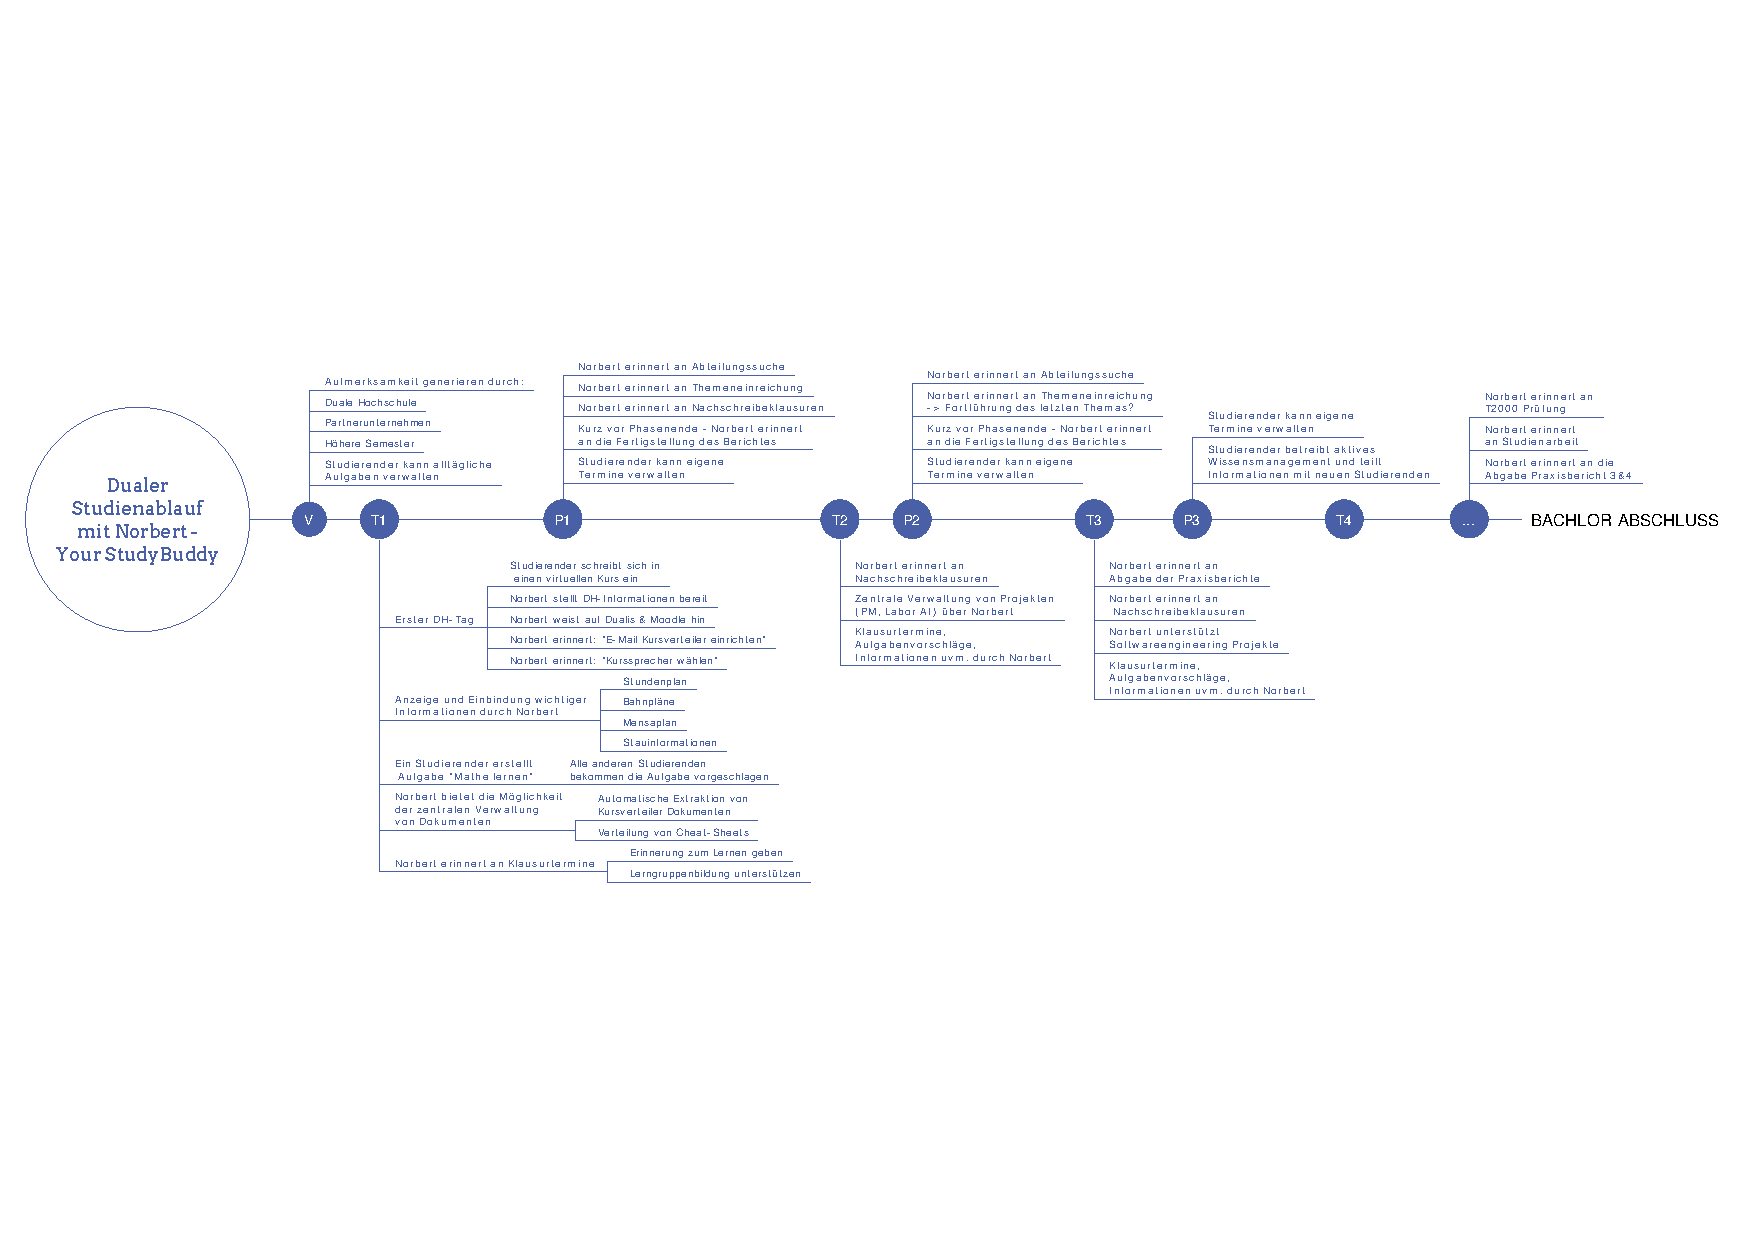
\includegraphics[scale=0.75]{images/timeline.pdf}
	\end{figure}

\end{landscape}
\newpage

\section{Nutzergruppen}

\subsection{Erstsemester-Studierender}
Ein Erstsemester-Studierender verfügt nur über relativ wenig Wissen, welche Aufgaben und Informationen er zum erfolgreichen Absolvieren des Studiums benötigt. Durch die Vorpraktikumsphase in den Partnerunternehmen werden zwar bereits einige Informationen vorab ausgetauscht, doch oftmals sind diese nicht sehr präzise und geraten schnell in Vergessenheit. Wichtige Termine und Fristen werden versäumt und die Vielzahl an Aufgaben in den ersten Semestern überfordern viele Studierende schnell. Zudem fehlen ihm oft die richtigen Informationen zu Beginn des Studiums. Nutzt der Studierende Norbert - Your StudyBuddy bereits zu Beginn des erstem Semesters - oder im sogar im Vorpraktikum - bekommt er vollautomatisch alle nötige Wissen zum Studium und die DHBW mitgeteilt. Weiterhin bekommt er sinnvolle Aufgaben und Termine aus vorherigen Jahrgängen vorgeschlagen und kann sich an ToDo's der Studienkollegen orientieren. Somit findet ein vollautomatische Wissensweitergabe statt. Durch dieses optimierte Wissens- und Aufgabenmanagement, welche speziell auf dual Studierende abgestimmt ist, hat der Studierende mehr Freizeit, die er für Hobbys, Kneipentouren und Partys nutzen kann.

\subsection{Erfahrene Studierende}
Studierende in den höheren Semestern nutzen die Anwendung nicht mehr hauptsächlich um einfach nur Informationen zu erhalten, sondern können über die Anwendung Aufgaben und Projekte verwalten. Außerdem können sie Wissen mit Erstsemester-Studierenden teilen. Somit profitieren die neuen Studierenden von den Erfahrungen  der vorherigen Semestern. Dabei geht die Wissensweitergabe teilweise komplett automatisiert vonstatten, sodass niemand zusätzlich \enquote{per Hand} Aufgaben und Informationen weitergeben muss. Die Integration von verschiedenen häufig genutzten Diensten ermöglicht Informationen in einer Anwendung zu bündeln und auf einen Blick darzustellen. Durch einen optimierten und strukturierten Studienalltag hat der erfahrene Studierende mehr Zeit zum bearbeiten von Projekten, Studienarbeiten und kann sich besser auf Prüfungen vorbereiten.